\chapter{Gestures}
Gestures are configurable robot movements, which mimic the human interactions with a touch panel. The available gestures depend on the robot model in use.

Gestures are executed via Python scripts using TnT Client Python package. Each gesture is a function that takes a varying number of parameters and the function execution returns when the motion is complete. See TnT Client reference manual for detailed description of the available parameters.

\warningbox{The software has very little parameter range validation and there is no collision detection in motion planning. Be very careful when performing gestures with given parameters and make sure the DUT is correctly positioned. It is always best to use low robot speed and acceleration when performing gestures for the first time or when changing parameters.}

\begin{figure}[h]
	\centering
	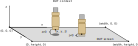
\includegraphics{dut_context.pdf}
	\caption{Illustration of DUT context. The x, y and z direction vectors define the DUT orientation in the embedding workspace.}
	\label{fig:dut_context}
\end{figure}

All gestures have a few common parameters. These are \emph{x}, \emph{y} and \emph{z} coordinates which determine the starting position of the gesture in DUT context. DUT context is a coordinate system where x and y define the "top left" corner of typical display where also the panel reports display coordinate (0, 0). The z-coordinate is zero at the DUT surface and increases upwards from the surface. This is illustrated in Figure \ref{fig:dut_context}. Robot will always first move to the given (x ,y, z) position before the actual gesture is performed. Typically the \emph{z} parameter can be omitted, in which case the DUT's \emph{base distance} is used as the z-coordinate. By default the base distance is 10 mm but it can be changed for each DUT by the user using TnT UI or TnT Client. Robot will move to the starting position using straight path from current position. This may cause collision if there are obstacles along this way. For this reason there is a gesture called \emph{jump} which safely moves robot over a DUT by going first to the maximum height. See section below for more details.

\begin{figure}[h]
	\centering
	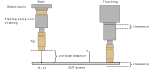
\includegraphics{gesture.pdf}
	\caption{Illustration of typical gesture motion and parameters.}
	\label{fig:gesture}
\end{figure}

Most gestures also have parameter \emph{clearance}, which is the z-coordinate in DUT context when the robot is touching the DUT. Clearance 0 will just barely touch the DUT surface while clearance -1 mm causes robot to press against the DUT when robot tries to move the effector 1 mm below the DUT surface. Most robot effectors have a spring or active voice coil which will flex during such motion. This is illustrated in Figure \ref{fig:gesture}. There is a limited amount of flex in the robot so user must be careful to position the DUT correctly and providing reasonable clearance value. Usually it is not advisable to make clearance more negative than -1 mm.

Most basic gestures also take \emph{azimuth} and \emph{tilt} parameters which are angles in degrees in the DUT context. These determine the orientation of the robot effector when the gesture motion is executed. Some robot models lack rotary joints to actually go to given orientation. In such case the parameter values are omitted by the trajectory planner.

Gesture motion takes into account the length of the tip currently attached to the robot tool head so that the effector touches the DUT surface in the same way with different tips. Usually a tip will make the tool roughly 13 mm longer than without tip. Tips can be changed automatically or manually but it is crucially important that the SW book-keeping of currently attached tip matches with the physical world. If for example user manually adds a tip to the robot but the software still thinks there is no tip attached, there is a risk of collision when gesture motion is performed.

Most parameters that affect gesture motion are given as parameters to gesture functions. However speed and acceleration are robot states which must be set using the robot API.


\section{One-Finger gestures}
This section describes the available gestures if the robot has one or more effectors.

\subsection{Jump}

Jump is used to move the robot effector over designated DUT from current position \emph{safely}. Given that direct route from current position over the DUT may be blocked by obstacles, the safest thing in general is to first go to maximum z-coordinate in the workspace context.

Jump will first move from current position to given \emph{jump\_height} if that position is higher than current position. If not, then current position is used as starting point. If jump heigh is not given, robot will rise to the highest possible position. This is the recommended way. After that, robot will move over the given DUT x, y -coordinates and finally go down to given DUT z-coordinate. Jump gesture is illustrated in Figure \ref{fig:tap_jump}

\notebox{It is always best to first jump over DUT e.g. to DUT coordinates (0, 0, 10) before executing any other gestures. Other gestures will just move from current location to the start of the gesture along straight path which poses risk of collision}.

\begin{figure}[h]
	\centering
	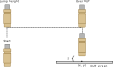
\includegraphics{jump.pdf}
	\caption{Illustration of the jump gesture.}
	\label{fig:tap_jump}
\end{figure}

Jumping over DUT top left corner can be performed with following Python script:

\begin{lstlisting}[language=Python]
from tntclient.tnt_client import TnTClient
client = TnTClient()
dut = client.dut("dut1")
dut.jump(x=0, y=0, z=10)
\end{lstlisting}

\subsection{Tap} 

During a tap gesture the robot first moves over the desired position on DUT at specified z-coordinate or base distance. After that the DUT taps the spot on DUT and returns back to the base distance. The tap duration i.e. how long the tip is in the lowest position can be adjusted. Please refer to Figure \ref{fig:tap_gesture} for illustration.

\begin{figure}[h]
	\centering
	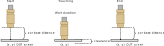
\includegraphics{Tap.pdf}
	\caption{Illustration of the tap gesture.}
	\label{fig:tap_gesture}
\end{figure}

Tap may be performed with the z-axis or by voice coil if robot has such device. Voice coil has a limited movement range so depending on the value of given z-coordinate or DUT base distance, robot may or may not need to first move the z-axis to get to the voice coil operation range. Voice coil has much higher maximum speed and acceleration than the z-axis so if tapping performance is important, user should use z-coordinate or base distance where the robot does not need to use the z-axis when performing consecutive taps.

Tapping DUT top left corner can be performed with following Python script:

\begin{lstlisting}[language=Python]
from tntclient.tnt_client import TnTClient
client = TnTClient()
dut = client.dut("dut1")
dut.tap(x=0, y=0, clearance=-1)
\end{lstlisting}

\subsection{Double tap}

Double tap is similar to tap gesture except that it taps the DUT surface two times. User can specify additional parameter \emph{interval} which is the time the robot waits at lifted position between the two taps. Note that the interval does not take into account the time it takes to move the finger up from the first tap and the time it takes to move the finger down for the second tap. 
Double tap is illustrated in Figure \ref{fig:double_tap_gesture}.

\begin{figure}[h]
	\centering
	\includegraphics{double_tap.pdf}
	\caption{Illustration of the double tap gesture.}
	\label{fig:double_tap_gesture}
\end{figure}

Double tapping the DUT top left corner with duration 1 s and interval 2 s can be performed with following Python script:

\begin{lstlisting}[language=Python]
from tntclient.tnt_client import TnTClient
client = TnTClient()
dut = client.dut("dut1")
dut.double_tap(x=0, y=0, clearance=-1, duration=1.0, interval=2.0)
\end{lstlisting}

\subsection{Multi tap}

Multi tap is a gesture that performs taps at multiple locations. User provides a list of points where each point is (x, y) position in DUT context where tap is performed. The same could be achieved with multiple calls to the normal tap gesture, but there is certain latency between execution of each tap due to trajectory calculations. If user wants to perform multiples taps consecutively as quickly as possible then multi tap is suitable.

Multi tap also takes parameter \emph{lift} which tells how high effector is lifted between taps.

Multi tapping the DUT at the four corners can be performed with following Python script:

\begin{lstlisting}[language=Python]
from tntclient.tnt_client import TnTClient
client = TnTClient()
dut = client.dut("dut1")
points = [TnTDutPoint(0, 0), TnTDutPoint(dut.width, 0), 
TnTDutPoint(dut.width, dut.height), TnTDutPoint(0, dut.height)]
dut.multi_tap(points=points, lift=2, clearance=-0.5)
\end{lstlisting}

\subsection{Watchdog tap}

Watchdog tap is basically the same as the tap gesture except that it is intended to be used with latency measurements which require a trigger signal from the exact time when the effector touches the DUT surface. There can be different triggering mechanisms but if the robot has voice coil, then the voice coil encoder changes are used as trigger. For this reason, watchdog tap z-motion is always done with the z-axis. Watchdog tap has \emph{trigger\_direction} parameter which can be used to determine whether trigger is signalled from "touch start" or "touch end".

Watchdog tapping the DUT top left corner with trigger signalled from touch start can be  performed with following Python script:

\begin{lstlisting}[language=Python]
from tntclient.tnt_client import TnTClient
client = TnTClient()
dut = client.dut("dut1")
dut.watchdog_tap(x=0, y=0, clearance=-1, trigger_direction="TOUCH_START")
\end{lstlisting}

\subsection{Spin tap}

Spin tap is the same as the tap gesture except that the effector spins around its axis during tap motion. User provides two angle parameter \emph{azimuth1} and \emph{azimuth2} which determine the spin angle when the effector starts to move down and when it reaches the clearance height, respectively. There is also additional boolean parameter \emph{spin\_at\_contact}. If set to true, the rotation happens only after the effector has reached the clearance height.

Spin tap can only be used with robots that have azimuth rotary joint.

Spin tapping the DUT top left corner with rotation of 90 degrees can be  performed with following Python script:

\begin{lstlisting}[language=Python]
from tntclient.tnt_client import TnTClient
client = TnTClient()
dut = client.dut("dut1")
dut.spin_tap(x=0, y=0, azimuth1=0, azimuth2=90, clearance=-1)
\end{lstlisting}

\subsection{Swipe} 
Swipe gesture consists of three separate parts: acceleration, swipe, and deceleration. The acceleration and deceleration are quarter circle arcs of specified radius. The greater the radius the more certain it is that the tip achieves the desired swipe speed (\textit{line drawing speed}) before it touches the DUT screen. Swipe motion is illustrated in Figure \ref{fig:swipe_gesture}a.

\begin{figure}[h]
	\centering
	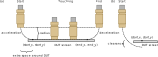
\includegraphics{Swipe.pdf}
	\caption{(a) Illustration of the swipe gesture. (b) Illustration of swipe arc motion when using negative clearance.}
	\label{fig:swipe_gesture}
\end{figure}

\warningbox{Robot may collide with DUT edges during swipe when using negative clearance parameter. Please read this section carefully before using swipe.}

Please note, that due to the arcs the DUT has to be positioned in such a way that the robot can move around it as indicated in Figure \ref{fig:swipe_gesture}a. Occasionally the screen might have high edges and the tip can hit them if the radius is too large. In this case, the user should use zero clearance and use smaller radius. If this does not work then drag gesture might be more appropriate (see Section \ref{sec:drag}). User should notice that the arc is formed towards the start point at the clearance height. Thus if clearance is negative and swipe is started at the very edge of the DUT, there is a risk of collision. This risk is pronounced when using large swipe radius or narrow  tip. This hazard is illustrated in Figure \ref{fig:swipe_gesture}b. It is good practice to start with small clearance such as -0.5 mm and test if it provides sufficient contact with the DUT screen. Sometimes the screens are not perfectly flat which may necessitate the use of more negative clearance values. Then it is best to reduce the swipe radius. Usually 6 mm radius is safe when using tip of diameter 10 mm and clearance -0.5 mm.

The swipe radius gives the robot room to accelerate to target speed so that during touch, the robot speed could be constant. The appropriate radius depends on several factors. Firstly, it may be limited by the collision risk i.e. if swipe starts at the very edge of the DUT and the tip is narrow, user may need to use radius of 6 mm or less. With robot that has voice coil, the arc motion is performed with voice coil which usually has movement range of roughly 9 mm. This also limits swipe arc radius.

The required swipe radius to achieve given speed depends mostly on the acceleration capability of each axis. The slowest axis sets the limit. Usually z axis and voice coil have very high maximum acceleration. Roughly 9000 mm/s$^2$ and 30000 mm/s$^2$ respectively. The x axis can typically reach acceleration of 3000 mm/s$^2$. Typically the y-axis is the slowest, reaching roughly 900 mm/s$^2$. Reaching swipe speed 250 mm/s requires roughly 25 mm swipe radius if acceleration is limited by the y-axis. Due to the difference in the axis accelerations, swipes can be done faster along robot x-axis than along y-axis.

%TODO: Add table and formulas for determining correct radius for different situations.

Swiping across DUT horizontally through the midpoint can be performed with following Python script:

\begin{lstlisting}[language=Python]
from tntclient.tnt_client import TnTClient
client = TnTClient()
dut = client.dut("dut1")
dut.swipe(x1=0, y1=dut.height/2, x2=dut.width, y2=dut.height/2, clearance=0, radius=6)
\end{lstlisting}

\subsection{\label{sec:drag}Drag}
Drag gesture is like swipe but without acceleration and deceleration parts. The tip goes first on top of the line starting point at the base distance. Then it goes directly down, draws the line, stops, and moves back up. With drag the speed might differ a lot during the line movement. However, is some cases with DUT with high/elevated edges or combinations with force measurements, drag is the only feasible option. Please refer to Figure \ref{fig:drag_gesture} for illustration.

\begin{figure}[h]
	\centering
	\includegraphics{Drag.pdf}
	\caption{Illustration of the drag gesture.}
	\label{fig:drag_gesture}
\end{figure}

Unlike swipe, drag allows user to specify pre-delay and post-delay to make robot wait until motion along DUT surface starts and until finger lifts off the surface at the end position.

Performing drag across DUT horizontally through the midpoint can be done with following Python script:

\begin{lstlisting}[language=Python]
from tntclient.tnt_client import TnTClient
client = TnTClient()
dut = client.dut("dut1")
dut.drag(x1=0, y1=dut.height/2, x2=dut.width, y2=dut.height/2, clearance=0)
\end{lstlisting}

\subsection{Multiswipe}

% TODO: Gesture should be renamed Multidrag to match other naming.

Multiswipe is the same as the drag gesture except that the robot performs given number of back-and-forth dragging movements on the DUT surface before lifting up. In addition to normal drag parameters, user specifies integer parameter \emph{n} to indicate how many drag movements are performed on the DUT. Value n=1 corresponds to normal drag gesture. Parameter n=2 moves effector from (x1, y1) to (x2, y2) and then back to (x1, y1) and then effector lifts up.

Making a multiswipe across DUT surface can be performed with following Python script:

\begin{lstlisting}[language=Python]
from tntclient.tnt_client import TnTClient
client = TnTClient()
dut = client.dut("dut1")
dut.multiswipe(x1=0, y1=dut.height/2, x2=dut.width, y2=dut.height/2, clearance=0, n=3)
\end{lstlisting}

\subsection{Circle}

In circle gesture the robot moves a circle path on the DUT surface. The given \emph{x}, \emph{y} coordinates define the starting point of the circle which is by default the right edge of the circle. User can specify the radius \emph{r} of the circle and the number of revolutions \emph{n}. The circle is by default done counter-clockwise but user can also set boolean parameter \emph{clockwise} to perform circle in clockwise direction. It is also possible to set parameter \emph{angle} to start the circle at some other point on the circle. The circle gesture is illustrated in Figure \ref{fig:circle_gesture}

\begin{figure}[h]
	\centering
	\includegraphics{circle.pdf}
	\caption{Illustration of the circle gesture.}
	\label{fig:circle_gesture}
\end{figure}


Performing circle gesture of radius 30 mm over two revolutions can be done with following Python script:

\begin{lstlisting}[language=Python]
from tntclient.tnt_client import TnTClient
client = TnTClient()
dut = client.dut("dut1")
dut.circle(x=0, y=0, r=30, n=2)
\end{lstlisting}

\subsection{Path}

In path gesture the robot effector moves on DUT through given list of (x, y, z) points along a polyline. Robot will accelerate and decelerate when going from one point to the next so that robot is at full stop at each point. Note that at each point, user can also specify \emph{z} coordinate in the DUT context so that it is possible to lift finger off the DUT surface during path motion. The path gesture is illustrated in Figure \ref{fig:path_gesture}.

\begin{figure}[h]
	\centering
	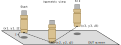
\includegraphics{path.pdf}
	\caption{Illustration of the path gesture.}
	\label{fig:path_gesture}
\end{figure}

Performing path gesture through points (0, 0, 10), (0, 0, 0) and (20, 20, 0) can be done with following Python script:

\begin{lstlisting}[language=Python]
from tntclient.tnt_client import TnTClient
client = TnTClient()
dut = client.dut("dut1")
points = [TnTDutPoint(0, 0, 10), TnTDutPoint(0, 0, 0), TnTDutPoint(20, 20, 0)]
dut.path(points=points)
\end{lstlisting}

\subsection{Smooth path}

Smooth path is the same as the path gesture except that the path connecting the given points is a third-degree spline that interpolates the given points. Unlike path gesture, the effector does not stop at the given points. It will accelerate to the set speed and travel at that constant speed along the spline path and finally decelerate to stop at the final point. The smooth path gesture is illustrated in Figure \ref{fig:smooth_path_gesture}.

\begin{figure}[h]
	\centering
	\includegraphics{smooth_path.pdf}
	\caption{Illustration of the smooth path gesture.}
	\label{fig:smooth_path_gesture}
\end{figure}

\warningbox{If the z-coordinates of the points are not the same, the spline path can go to unexpected z-values due to the way spline interpolation works. Path planner tries to detect such unintentional points and raise an error.}

Performing a smooth path gesture through points (0, 0, 0), (20, 0, 0) and (20, 20, 0) can be done with following Python script:

\begin{lstlisting}[language=Python]
from tntclient.tnt_client import TnTClient
client = TnTClient()
dut = client.dut("dut1")
points = [TnTDutPoint(0, 0, 0), TnTDutPoint(20, 0, 0), TnTDutPoint(20, 20, 0)]
dut.smooth_path(points=points)
\end{lstlisting}

\section{Force gestures}

Force gestures are movements on DUT where robot applies given amount of force on the DUT. In standard robots equipped with voice coil the force is generated by moving the effector against DUT with the voice coil until target force is reached. The force is then applied in the direction of the voice coil axis which should typically be close to the normal direction of the DUT plane.

There are two ways to produce force with voice coil: \emph{open loop force control} and \emph{closed loop force control}. Two-finger Synchro robots support only open loop force control. One finger force actuator robots support either open loop or closed loop force control, depending on usage, and selected HW options.

Open loop control is based on the observation that the current draw of the axis is proportional to force. Hence we can construct a look-up table of current-force values by pressing against a reference scale. Then for given target force, the maximum current draw of the axis is set to corresponding value from the table and the effector is pressed against DUT until the current saturates. The look-up table is calibrated once as part of robot setup and then used by gestures later.

% TODO: Here it would be nice to show some plots of curret vs force and also a plot to illustrate the accuracy of open and closed loop force.

Closed loop control is based on active force feedback coupled to the voice coil motion controller. Usually \emph{loadcell} integrated to the axis is used as such feedback device.  Software can then set the axis to move until given force is reached according to the force feedback. The specified force can further be calibrated against a scale to produce a force-force look-up table.

Closed loop force is more accurate than open loop force but it requires dedicated hardware, and is slower to perform due to feedback based active adjustment.

% TODO: Any other characteristics of open loop / closed loop to mention here?

Force calibrations are performed as part of robot delivery using OptoFidelity Force audit and calibration block accessory. User can also perform the calibrations using the Force calibration view in TnT UI in case the calibration becomes invalid for some reason such as change of a hardware part. See Section \ref{sec:force_calibration} for more details.

In the force gesture API force is expressed in \emph{grams of force} denoted gF. It can be converted to Newtons by 1000 gF = 9.80665 N.

\subsection{Press}

Press gesture is similar to tap except that the z motion is planned so that given amount of force is applied on the DUT. User provides parameter \emph{force} to specify how many grams of force is applied on the DUT.

\begin{figure}[h]
	\centering
	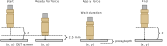
\includegraphics{open_loop_press.pdf}
	\caption{Illustration of the open loop press gesture.}
	\label{fig:open_loop_press_gesture}
\end{figure}

When using open loop force system, user can specify parameter \emph{press\_depth} which is the z-coordinate in DUT context where the effector is attempted to be moved using position control mode. Once the effector hits the DUT surface the voice coil current draw starts to increase until it saturates to the value corresponding to the specified force. The default value of press\_depth is -1 which should normally be sufficient. This parameter has only effect in open loop force mode. Before voice coil is moved, the z-axis is moved so that the effector z-coordinate in DUT context is 2.5 mm. This is to guarantee that the voice coil current saturation works consistently. Open loop press gesture is illustrated in Figure \ref{fig:open_loop_press_gesture}.

\begin{figure}[h]
	\centering
	\includegraphics{closed_loop_press.pdf}
	\caption{Illustration of the closed loop press gesture.}
	\label{fig:closed_loop_press}
\end{figure}

When using closed loop force system, the press\_depth parameter is not used because the voice coil firmware is set to force control mode instead of position control. Before force application, the robot performs force tare where the force feedback is zeroed while the effector is not touching the DUT. After tare is complete, the effector is moved to close contact with the DUT surface. Then the voice coil is set to force control mode to apply the given force using closed loop control. The effector must be in contact with the surface when the mode is switched to force control to avoid significant initial overshoot in force. Closed loop press gesture is illustrated in Figure \ref{fig:closed_loop_press}.

Following script can be used to perform press against DUT at DUT xy-origin applying 500 grams of force:

\begin{lstlisting}[language=Python]
from tntclient.tnt_client import TnTClient
client = TnTClient()
dut = client.dut("dut1")
dut.press(x=0, y=0, z=10, force=500, press_depth=-1)
\end{lstlisting}

The API works the same with open and closed loop force except the latter ignores the press\_depth parameter.

\subsection{Drag force}

Drag force is similar to the drag gesture except that a specific force is applied on the DUT while the finger drags over the DUT surface. User provides parameter \emph{force} to specify how many grams of force is applied on the DUT. 

Considering the nature of drag force, there is no guarantee of the applied force being accurate throughout the gesture. During drag, the robot finger is moving along the surface, and for example changes in friction, or inconsistencies in the surface may affect the force momentarily. Generally drag force is more accurate with lower speeds, as the system has more time to adjust to changes.

\begin{figure}[h]
	\centering
	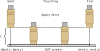
\includegraphics{drag_force_open_loop.pdf}
	\caption{Illustration of the open loop drag force gesture.}
	\label{fig:open_loop_drag_force}
\end{figure}

With open loop system the finger is attempted to be moved at clearance -2 mm while the voice coil current value saturates to the value that corresponds to given force. Open loop drag force gesture is illustrated in Figure \ref{fig:open_loop_drag_force}.

\begin{figure}[h]
	\centering
	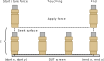
\includegraphics{drag_force_closed_loop.pdf}
	\caption{Illustration of the closed loop drag force gesture.}
	\label{fig:closed_loop_drag_force}
\end{figure}

With closed loop force, the robot first moves to base distance or given z-height and performs force tare. Then it will move the effector to touch the surface and change voice coil to force control mode. The effector will then perform normal drag motion in xy-direction while the voice coil axis applies force in closed force control loop. At the end of the drag, the control mode is changed back to position mode and the finger rises to base distance or given z-height. Closed loop drag force gesture is illustrated in Figure \ref{fig:closed_loop_drag_force}.

Following script can be used to perform drag force against DUT over DUT width applying 500 grams of force:

\begin{lstlisting}[language=Python]
from tntclient.tnt_client import TnTClient
client = TnTClient()
dut = client.dut("dut1")
dut.drag_force(x1=0, y1=dut.height/2, x2=dut.width, y2=dut.height/2, z=10, force=500)
\end{lstlisting}

The API works the same with open and closed loop force.

\section{Two-finger gestures}

This section describes the available gestures if the robot has at least two fingers. Usually these are performed with OptoFidelity Synchro tool which can rotate two fingers around the robot z-axis and the fingers can be synchronously separated along an axis that is perpendicular to the rotation axis.

\subsection{One-finger gestures with two-finger robot}

It is possible to use all the one-finger gestures with two-finger robot. With Synchro finger robot, it is possible to specify additional parameters to control how the gestures are performed. 

\begin{figure}[!h]
	\centering
	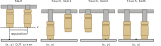
\includegraphics{two_finger_gestures.pdf}
	\caption{Illustration of one-finger gestures with two-finger robot. Notice where the target location (x,y) is in each case.}
	\label{fig:two_finger_gestures}
\end{figure}

User can give parameter \emph{separation} to specify what the finger axis-to-axis separation will be while the gesture is performed. This usually only matters if both finger effectors are used during the gesture. If the parameter is not given, a default separation value is used. This is normally the home separation.

With parameter \emph{tool\_name}, user can specify which finger is used to perform the gesture. Valid values are "tool1", "tool2" and "both". Default value is "tool1" corresponding to the default finger in the Synchro tool. With value "tool2" the second finger performs the tap motion and by default the second finger is moved over the specified location. With value "both" both fingers perform the gesture simultaneously (e.g. tap becomes two-finger tap). In that case the mid point between the two fingers is moved over the given tap location.

It is also possible to specify parameter \emph{kinematic\_name} to control which kinematics is used to plan the motion. Currently this is only implemented for the tap gesture. Valid values are "tool1", "tool2", "mid" and "synchro". This essentially means that user can control which point on the robot is moved to the location specified by the gesture coordinates. Value "tool1" moves the first finger, value "tool2" moves the second finger, value "mid" moves the mid point between the fingers and value "synchro" moves the mount point of the Synchro tool. This parameter makes it possible to e.g. tap with both fingers but let the tap location be specified with finger 1 instead of the mid point which is the default in the absence of \emph{kinematic\_name}. Figure \ref{fig:two_finger_kinematic_name} and the script below illustrate such use case.

\begin{figure}[!h]
	\centering
	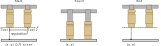
\includegraphics{two_finger_kinematic_name.pdf}
	\caption{Illustration of performing tap with \emph{kinematic\_name} "tool1" and \emph{tool\_name} "both".}
	\label{fig:two_finger_kinematic_name}
\end{figure}

\begin{lstlisting}[language=Python]
from tntclient.tnt_client import TnTClient
client = TnTClient()
dut = client.dut("dut1")
dut.tap(x=dut.width/2, y=dut.height/2, separation=60, tool_name="both", kinematic_name="tool1")
\end{lstlisting}

These gestures and parameters are illustrated in Figure \ref{fig:two_finger_gestures}.

\warningbox{When using two-finger gestures or one-finger gestures with the second or both fingers, make sure that both fingers have tip attached. Also the software book-keeping of attached tips must match reality. Otherwise there is risk of collision. See Figure \ref{fig:two_finger_collision} for illustration.}

\begin{figure}[!h]
	\centering
	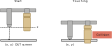
\includegraphics{two_finger_collision.pdf}
	\caption{Illustration of possible collision with two-finger robot if asymmetric tip configuration is used.}
	\label{fig:two_finger_collision}
\end{figure}

\subsection{Pinch}

In pinch gesture, the mid point between the two fingers is moved over given xy position so that both fingers are at specified z-coordinate or base distance. After that both fingers are moved at given clearance to touch the DUT surface. Then the fingers move from given start separation \emph{d1} to end separation \emph{d2}. Finally both fingers are lifted to the given z-position or base distance. Pinch gesture is illustrated in Figure \ref{fig:pinch}.

Notice that this gesture can perform \emph{pinch} and \emph{zoom} type motions depending on the given separation parameters.

\begin{figure}[h]
	\centering
	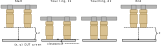
\includegraphics{pinch.pdf}
	\caption{Illustration of the pinch gesture.}
	\label{fig:pinch}
\end{figure}

Following script can be used to perform pinch over DUT from separation 60 mm to 30 mm at the center of DUT using azimuth angle 45 degrees:

\begin{lstlisting}[language=Python]
from tntclient.tnt_client import TnTClient
client = TnTClient()
dut = client.dut("dut1")
dut.pinch(x=dut.width/2, y=dut.height/2, d1=60, d2=30, azimuth=45)
\end{lstlisting}

\subsection{Rotate}

In rotate gesture, the mid point between the two fingers is moved over given xy position so that both fingers are at specified z-coordinate or base distance. After that both fingers are moved at given clearance to touch the DUT surface. Then the fingers rotate from given \emph{azimuth1} angle to \emph{azimuth2} angle. Finally both fingers are lifted to the given z-position or base distance. Rotate gesture is illustrated in Figure \ref{fig:rotate}. 

\begin{figure}[h]
	\centering
	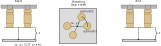
\includegraphics{rotate.pdf}
	\caption{Illustration of the rotate gesture.}
	\label{fig:rotate}
\end{figure}

Following script can be used to perform rotate gesture over DUT from azimuth angle 0 degrees to azimuth angle 90 degrees at the center of DUT using separation 60 mm:

\begin{lstlisting}[language=Python]
from tntclient.tnt_client import TnTClient
client = TnTClient()
dut = client.dut("dut1")
dut.rotate(x=dut.width/2, y=dut.height/2, azimuth1=0, azimuth2=90, separation=60)
\end{lstlisting}
